\section{RDOS} \label{s:rdos}
The challenges of creating a relational \os{} are multiple and substantial. The first deals with the most basic question of how do we obtain needed \md{} in the first place (\S\ref{s:om}). To solve this we need to begin with a definition of what is needed (\S\ref{s:def}). We can then move on to the problem of how to extract and affine this \md{} to the associated data object (\S\ref{s:mxe}), how to create relations (\S\ref{s:cr}), how to persist these relations (\S\ref{s:pr}), and finally to put this information to good use through modeling and analytics (\S\ref{s:models}).


\subsection{Obtaining Metadata} \label{s:om}
To date there is relatively little metadata being associated with the data objects in object stores.  There are a number of reasons for this.

\textbf{Application Reluctance}: Legacy \apps{} were built before a time when there was a well-defined means for storing and associating \md{} with data objects. However, even in the presence of such mechanisms today, a paucity of \md{} persists. First, a general \app{} by itself is unlikely to know what constitutes salient \md{} for a given file. Second, most commercial \apps{}, recognizing the value of \md{} to the customer, are reluctant to give up control of the \md{} to be used outside the confines of the application itself. Commercial \app{} providers may not be motivated to put extensive \md{} into a data store as it allows the customer to detach the data from the \app{}, in the process reducing the stickiness of the \app{}. This creates a financial disincentive to allow the user free and ready access to this \md{} without the need to involve the creating \app{}.

Further, even if a commercial \app{} provider is properly motivated to do so for the good of the customer, it's hard to determine what is the right set of data to include in \md{} as each customer is different. Just as with a RDBMS, where individual customers create relations amongst data sets as appropriate to their own needs, the customer needs to be able to define the \md{} that is apropos to their specific environment.

\textbf{Tools for Association}: Few tools exists to enable the systematic association of metadata to data objects.  Business agents with the necessary domain expertise for determining what constitutes relevant \md{} are unlikely to have the technical expertise required for tool development.

\textbf{Sophisticated Metadata Stores}: Even when modern \apps{} wish to associate meaningful \md{} with data objects, few \oss{} have the sophistication to provide the necessary foundation for good programming practice.

For example, for \md{} to be a first-class entity it's necessary that we are able to partition the address space so that different users can create, modify and delete their own \md{} in isolation. Today, most systems provide a single bucket where all \md{} is housed. Changes by one user therefore affect every other user, often in unpredictable ways. To protect user data from such unintended manipulations, all data stores partition the address space for data objects; few provide equivalent functionality for \md{}. For these reasons HCP allows \md{} partitions for each data abject. Figure \ref{fig:object} illustrates this concept with a data object that has eight distinct \md{} partitions. In \S\ref{s:mxe} we prescribe a mechanism for users to populate these \md{} partitions for both new data ingest, as well as for existing objects already stored.

\begin{figure}[h]
  \centering
    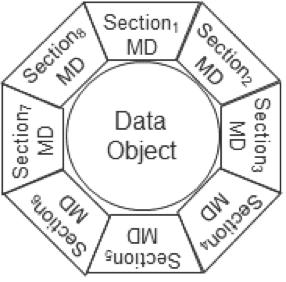
\includegraphics[width=0.25\textwidth]{fig/object.png}
  \caption{Object with Metadata Partitions}
  \label{fig:object}
\end{figure}

Finally, it's critical that an \os{} can scale---not just in its ability to store petabytes of data, but to be able to keep track of billions of discrete objects and associated \md{}. The former is comparatively easy, the latter is far more difficult. With HCP, each node can independently manage in excess of 800 million data objects and associated \md{}, a full cluster can manage 64 billion.


\subsection{Defining} \label{s:def}
The first step is to define what \md{} should be extracted or applied to data objects. Search engines can crack many file types and extract not only data from the core file, but also in some cases \md{} embedded in the file's header (e.g. in the case of DICOM images). However, standard data is is made far more useful by applying \emph{semantic meaning} to the content. This step is difficult for a general search engine to do as, by its very nature, semantic meaning is often particular to a user or organization and therefore doesn't lend itself to a generic solution.

Creating an ontology, where semantic meaning can be mapped to data, is referred to as a \emph{Data Dictionary}. Multiple such dictionaries can be created, each with meaning peculiar to a function within an organization. For example, one dictionary may contain a grammar common to a particular vertical, such as the field of healthcare, while other dictionaries will be particular to the organization itself, such as codenames used within a company. The sum of the individual data dictionaries creates the compendium necessary to inform the extraction and application step.


\subsection{Extraction / Application} \label{s:mxe}
The data dictionaries defined in the prior step act as \emph{extractors} or \emph{applicators} run across a field of previously ingested data objects or against individual objects during ingestion. When applied as a filter, objects are scanned for relevant key-value pairs within the data object with the results applied as \md{} scalars. Of course, such extraction is only possible where the data object is searchable. In cases where it is not, such as for image files, applicators would apply \md{} as defined in the data dictionaries to relevant data objects.

Since there can be multiple dictionaries, an object $O$ is run through a pipeline of size $p$ where the rules of each dictionary $d$ are applied in turn. For extraction operations we have $f_1 = \sum_{i=1}^p O \cap d_i$, for applicator operations we have $f_2 = \sum_{i=1}^p O \cup d_i$. In cases where a particular step in the pipeline has no rules to apply against an object that step becomes the identity function, that is $O_{input} = O_{output}$. Note that while it's possible that every step in a pipeline will be exclusively of type $f_1$ or $f_2$, this is not requirement; that is, $f_1$ and $f_2$ are not mutually exclusive.

Once run through the pipeline, data objects are coupled with relevant \md{} and stored as scalars, which can be used for subsequent queries by client \apps{} and to inform relations between objects.

\begin{figure}[h]
  \centering
    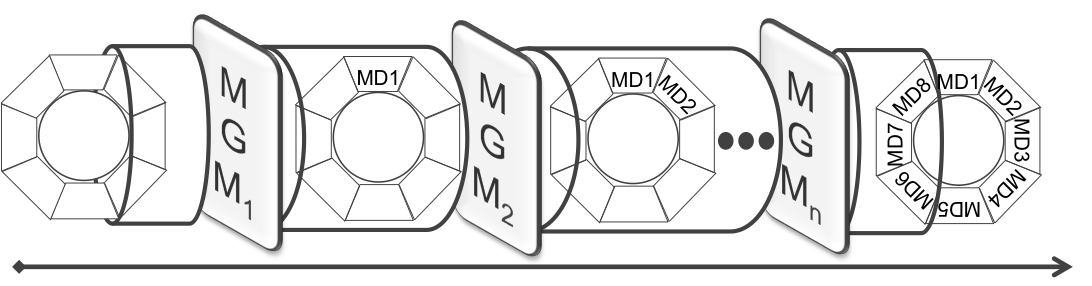
\includegraphics[width=\linewidth]{fig/md-pipe.png}
  \caption{Metadata Generation Pipeline}
  \label{fig:pipe}
\end{figure}

In this model the extraction or application steps in the pipeline are referred to as a \emph{\md{} generation module}, or MGM. As depicted in Figure \ref{fig:pipe}, a data object progresses through a series of MGMs, where an MGM comprises a script language specific to the task. At every stage a decision is made whether there is \md{} to be applied. While each MGM is independent, the ordering of MGMs can matter as the algorithm applied at any individual MGM may base a decision of whether to add, change or delete a \md{} section based not only the data object itself, but rather the union of the data object and \md{} accumulated in the pipeline to that point. Nonetheless, fundamental to this design is that an MGM is independent, to allow the flexibility of adding or updating MGMs in existing pipelines.

In HCP the address space is partitioned into \emph{namespaces} that essentially act as a virtual instance of the system as a whole. This segregation allows different data management and access policies to be applied to each set of data objects housed within a particular namespace.  It is a natural extension that each namespace may have a different set of MGMs to analyze data objects specific to a namespace (Figure \ref{fig:mgp}). This allows finer-grain decisions to applied to objects already grouped by user.

\begin{figure}[h]
  \centering
    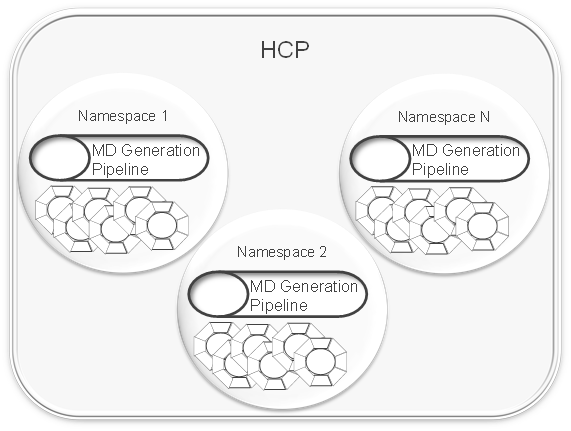
\includegraphics[width=\linewidth]{fig/cluster-mgp.png}
  \caption{Unique Pipeline per Namespace}
  \label{fig:mgp}
\end{figure}

Database programmers likely recognize that the MGM construct is conceptually similar to a \emph{stored procedure} in a RDBMS. A stored procedure is a subroutine stored in the \db{} data dictionary that runs on the \db{} server itself rather than directly on the client. In this model the MGM acts as a stored procedure, where common code can be run directly on the RDOS cluster rather than the client.

Note that a client \app{} could choose to perform all the functions of the MGM pipeline directly by reading an object, applying \md{}, and then rewriting this object back to the RDOS cluster. The downside of this method is that network bandwidth is consumed by the roundtrip for the read/write operations. It can therefore be more efficient to perform this same function on the cluster by running objects through the MGM pipeline. MGM scripts can be created either by the \app{} provider or constructed by the system administrator through a GUI.

\subsection{Creating Relations} \label{s:cr}
Armed with the \md{} from \S\ref{s:mxe} we move to the next step of using this \md{} to create relations among objects. For this discussion we use the example of an auto insurance company servicing a customer claim after a vehicle collision. We have three components to the claim: the claim form, digital photographs taken by the appraiser of the damage sustained, and a scan of the police report. These rich data types are good candidates for an \os{} as all are \ud{}.

Traditional \apps{} create a \db{} to collect transactions and create a schema to associate\db{} tables with one another. However, mobile \apps{} may not wish to require a local \db{}, instead choosing a remote \db{} for this function. In \S\ref{s:uddb} we state that \oss{} are a \db{} for \ud{}. Here RDOS acts as the \db{} for both the scalar data (in the form of key-value \md{} tags) and the data objects (blobs), which consist of any arbitrary file type. To use RDOS in our insurance example we begin with the claim form where a Claim ID (\texttt{CID}) is assigned (\texttt{CID=1234}) and ingested into RDOS. Subsequently the photos from the appraiser and the scan of the police report are uploaded. For all objects there is a \md{} tag set where \texttt{CID=1234}, providing a common key amongst the objects. At ingest, the client \app{} can choose to add a second \md{} field indicating that the images are related to the claim form. As objects are identified by URI, this translates to: \texttt{RelTo=URI\{Object1\}}. Through this structure we have a means of relating the full set of objects which are all associated with the same insurance claim.

This example depends upon the \app{} explicitly creating the relation between the objects by setting the \texttt{RelTo} \md{} tag, which is the preferred method for new object ingest. However, the same mechanism described in \S\ref{s:mxe} for adding \md{} to objects already stored can be applied here. The final stage of a MGM pipeline can be used to assign the relationship tag to objects in the same manner as all other \md{}. The difference in this final MGM script is that it must persist all \md{} tags found when enumerating over a set of existing objects. The system administrator can then define how these objects are to be related via a GUI, which in turn creates the needed MGM script.

\subsection{Persisting Relations} \label{s:pr}
Once we've done the hard work of extracting key \md{} and presenting mechanisms to the user (both human and application) to define relations, we need to select a means of persisting these relations in a manner that makes sense for the data type. In our model we have chosen a \gdb{} for this function as the graph model provides an excellent means of describing relation. Graph database models can be defined as those in which data structures for the schema and instances are modeled as graphs or generalizations of them, and data manipulation is expressed by graph-oriented operations and type constructors \cite{Angles:2008:SGD:1322432.1322433}.

Graph databases are described as ``whiteboard friendly.'' Drawing circles and connecting them with lines on a whiteboard is how we visualize graphs. We denote data points as \emph{nodes} and connect (relate) nodes with \emph{links}\footnote{Graph theory is a branch of discrete mathematics. Nodes are referred to as \emph{vertices} and what we call links are referred to as \emph{edges}, where edges connect pairs of distinct vertices. A simple graph (such as we'll be using in our descriptions) with $V$ vertices has at most $V(V-1)/2$ edges. We won't be dealing with graphs mathematically other than to note that a graph is defined by its vertices and its edges, not by the way we choose to draw it \cite{DBLP:books/daglib/0001826}.}, as illustrated in Figure \ref{fig:epi} (p. \pageref{fig:epi}). Graph databases, such as NEO4j \cite{Webber:2012:PIN:2384716.2384777}, are well suited to \ud{} as they are typeless and have no set schema, while providing several advantages for our application.

First, the graph data model is useful when the interconnectivity of data and the ability to discover the \emph{relationships between values} is important, rather than simply commonality \emph{among value sets} typical to relational models. Discovering relations is fundamental to our design, so its important we select a data structure that can readily describe relations with good performance. Unlike join operations in relational databases or map-reduce operations in other databases, graph traversals are in constant time \cite{redmond2012seven}. Graph databases make it easy to discover centrality, where we measure individual nodes against a full graph. (The most famous centrality algorithm is Google PageRank \cite{ilprints422}. In \S\ref{s:models} we use centrality in an epidemiology example.) Finally, graph databases have been shown to perform full-text character searches significantly faster than relational databases \cite{Vicknair:2010:CGD:1900008.1900067}.

Popular examples of publicly available \apps{} that make use of graph databases include Freebase\footnote{\href{http://www.freebase.com}{http://www.freebase.com}} and the Disease Ontology database\footnote{\href{http://disease-ontology.org}{http://disease-ontology.org}}. Freebase, created by Metaweb and acquired by Google in 2010, is a large community \md{} \db{} described as ``an open shared database of the world's knowledge.'' Disease Ontology, created by the University of Maryland School of Medicine, represents a comprehensive knowledge base of 8043 inherited, developmental and acquired human diseases \cite{schriml2012disease}.

\subsection{Models and Analytics} \label{s:models}
Once the data is available and programmatically accessible through well-defined APIs, modeling types that users can perform can be considered.

Object associations can be definitive or manufactured through a probabilistic generative model to guide inference from incomplete data.  The former can be prescribed by the user by linking objects through a GUI or template; the latter through Bayesian inference \cite{Pearl:1988:PRI:52121}, which provides a rational framework for updating beliefs about latent variables in generative models given observed data \cite{MacKay:2002:ITI:971143}.

Creating Bayesian models through graphs and predicate logic is more commonly the domain of data scientists than IT users. However, the goal for our system isn't to mandate a specific model of relation (definitive or derived), but rather to take care in design to not implicitly restrict the user to a particular model. Our system must provide the flexibility to persist and mutate object relation to meet a variety of user requirements\footnote{Nate Silver discusses the breadth of problems to which Bayesian reasoning can be applied in \cite{silver2012signal}.}.

As such, our goal is to provide an abstract framework over which schemas can be applied with sufficient flexibility to allow these relations to span the prosaic, e.g. linking monotonically increasing instances of an object (creating a version tree), to the expressive, e.g. a graph schema where nodes represent variables and directed edges between nodes represent probabilistic causal links.

For example, in an epidemiology study nodes might represent whether a patient has a cold, a cough, a fever or other conditions, and the presence or absence of links indicates that colds tend to cause coughing and sinus inflammation but not fever; sinus inflammation tends to cause headache but not fever; and so on \cite{tenenbaum2011grow}. The probability of a causal relation can be further refined by applying a weighting (0 - 1.0) to each link; e.g. there's a 60\% likelihood that a cold will result in a cough. As depicted in Figure \ref{fig:epi} graphs provide a ready means for users to interpret data and visualize relationships.

\begin{figure}[h]
  \centering
    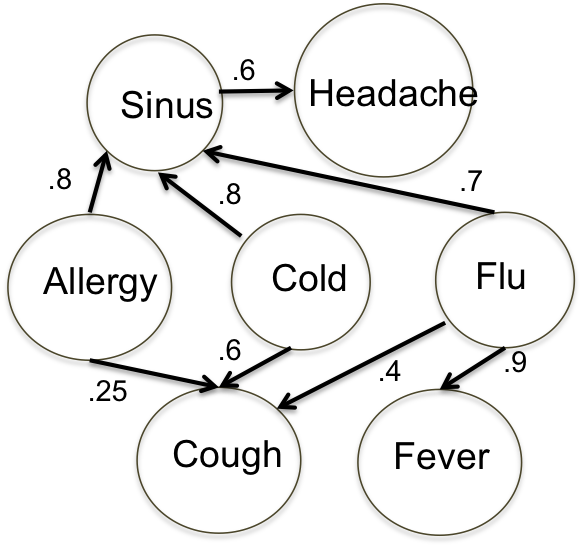
\includegraphics[width=0.3\textwidth]{fig/disease-graph.png}
  \caption{Epidemiology Directed Graph}
  \label{fig:epi}
\end{figure}

Through the proper application of multi-predicate constraints over the field of objects in a domain, the user is able to resolve to \emph{classes} of objects---such as all objects associated with the progenitor of a disease. For example a user might want to view all outcomes for patients over 60 in Africa with diminished respiratory function in the presence of the bacteria Legionella, and contrast this to those in the presence of the virus adenovirus to determine whether better outcomes are seen in patients with bacterial versus viral pneumonia.

Such analytic questions can be compute intensive when run over the full mass of \ud{} (what we refer to as \emph{data objects} in \S\ref{s:obj}), but are comparatively lightweight operations when run against the much smaller set of \md{} associated with these data objects. Here the \md{} acts an abbreviation of the objects and allows us to create information from an otherwise undistinguished data mass.

